\let\negmedspace\undefined
\let\negthickspace\undefined
\documentclass[journal]{IEEEtran}
\usepackage[a5paper, margin=10mm, onecolumn]{geometry}
%\usepackage{lmodern} % Ensure lmodern is loaded for pdflatex
\usepackage{tfrupee} % Include tfrupee package

\setlength{\headheight}{1cm} % Set the height of the header box
\setlength{\headsep}{0mm}     % Set the distance between the header box and the top of the text

\usepackage{gvv-book}
\usepackage{gvv}
\usepackage{cite}
\usepackage{amsmath,amssymb,amsfonts,amsthm}
\usepackage{algorithmic}
\usepackage{graphicx}
\usepackage{textcomp}
\usepackage{xcolor}
\usepackage{txfonts}
\usepackage{listings}
\usepackage{enumitem}
\usepackage{mathtools}
\usepackage{gensymb}
\usepackage{comment}
\usepackage[breaklinks=true]{hyperref}
\usepackage{tkz-euclide} 
\usepackage{listings}
% \usepackage{gvv}                                        
\def\inputGnumericTable{}                                 
\usepackage[latin1]{inputenc}                                
\usepackage{color}                                            
\usepackage{array}                                            
\usepackage{longtable}                                       
\usepackage{calc}                                             
\usepackage{multirow}                                         
\usepackage{hhline}                                           
\usepackage{ifthen}                                           
\usepackage{lscape}
\usetikzlibrary{angles, quotes}
\begin{document}

\bibliographystyle{IEEEtran}
\vspace{3cm}

\title{9.5.3}
\author{EE24BTECH11055 - Sai Akhila Reddy Turpu}
% \maketitle
% \newpage
% \bigskip
{\let\newpage\relax\maketitle}

\renewcommand{\thefigure}{\theenumi}
\renewcommand{\thetable}{\theenumi}
\setlength{\intextsep}{10pt} % Space between text and floats


\numberwithin{equation}{enumi}
\numberwithin{figure}{enumi}
\renewcommand{\thetable}{\theenumi}

% Question
\section*{Question:}
\begin{align}
\frac{dy}{dx} + \frac{y}{x} = x^2
\end{align}
%  Solution
\section*{Using Finite Differences to solve the given Differential Equation: }
The finite difference method is a numerical technique for solving differential equations by approximating derivatives with differences.
The first forward difference approximation of the derivative of $f(x)$ at $x$ is given by:
%This is forward difference, there are variations like backward difference, central differences also...
\begin{align}
    \frac{dy}{dx}&=\frac{f(x+h)-f(x)}{h}
\end{align}
Let $f(x+h)=y_{n+1}$ and $f(x)=y_n$
\begin{align}
    \implies y_{n+1}&=h\times\frac{dy}{dx}+y_n\\
    \implies y_{n+1}&=h\brak{x^2-\frac{y}{x}}+y_n
\end{align}
We already know that our derivative is given by:
\begin{align}
\frac{dy}{dx}&=x^2-\frac{y}{x}
\end{align}
Let's assume the intial conditions to be: $x_0=1$ and $y_0=0.25$
The derivative at the initial conditions can be caluculated by substituting $x_0$ and $y_0$ in equation $(1)$.\\
\begin{align}
\frac{dy}{dx}|_{x=x_0}=1-0.25 =0.75
\end{align}
%Let's assume an infinitesimally small number h, for the approximation
Let $h=10^{-3}$ and $f_1(x)=f(x+h)$\\\\
We get $f_1(x)=f(x)+h\times\frac{dy}{dx}|_{x=x_0} $\\\\
$f_1(x)=0.25+10^{-3}\times0.75=0.25075$\\
Thus, $x_1=x_0+h=1+10^{-3}=1.001$,\\$y_1=y_0+h\times\frac{dy}{dx}|_{x=x_0}=0.25075$\\\\
What we've essentially done is, obtaining a point which is very close to the initial point along the direction of the derivative at that point.\\To obtain the entire curve we repeat the process consecutively.\\For finding $f_2(x)$, find $\frac{dy}{dx}|_{x=x_1}$ using equation $(1)$ and substitute it in equation $(2)$ Find $f_2(x), f_3(x)$ and so on and plot the points to get the curve.
%We get the curve to be y=(x^3)/4
\section*{JEE Method:}
\begin{align}
    \frac{dy}{dx}+\frac{y}{x}=x^2
\end{align}
Finding the Integrating factor:
\begin{align}
e^{\int \frac{1}{x} \, dx} &=e^{\ln{x}}=x\\
\text{Thus } IF &= x \\
y(x)&=\int x^2\times x\, dx\\
y.x &= \frac{x^4}{4}+C    
\end{align}
Let's assume $C=0$, we get:\\
\begin{align}
    y=\frac{x^3}{4}
\end{align}
We can now verify that the given graph is $y=\frac{x^3}{4}$


\begin{figure}[h]  % 'h' specifies the preferred position for the figure (here, 'h' means "here")
  \centering  % Centers the figure
  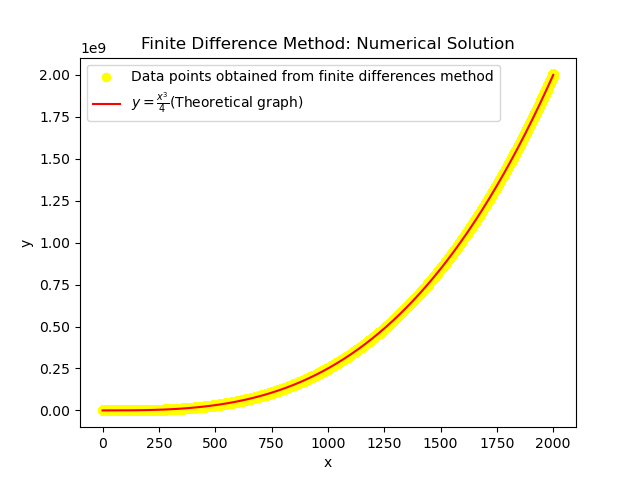
\includegraphics[width=\columnwidth]{figs/de1.png}  
  \caption{$y=\frac{x^3}{4}$}
  \label{fig:example}  % Label for referencing
\end{figure}


\end{document}
